\documentclass[11pt]{article}
\usepackage[a4paper,margin=28mm]{geometry}
\usepackage{amsmath,amssymb,amsthm,mathtools,booktabs,microtype,graphicx}
\usepackage{placeins}
\usepackage[T1]{fontenc}
\usepackage{lmodern}
\usepackage[hidelinks]{hyperref}
\hypersetup{pdftitle={Singular weights and operator dependence in matrix-valued transport},pdfauthor={Weiyan WU}}
\newtheorem{theorem}{Theorem}[section]
\newtheorem{proposition}[theorem]{Proposition}
\newtheorem{lemma}[theorem]{Lemma}
\newtheorem{corollary}[theorem]{Corollary}
\theoremstyle{definition}
\newtheorem{example}[theorem]{Example}
\newtheorem{remark}[theorem]{Remark}
\DeclareMathOperator{\tr}{tr}
\DeclareMathOperator{\sym}{sym}
\DeclareMathOperator{\Ran}{Ran}
\DeclareMathOperator{\diag}{diag}
\DeclareMathOperator{\CE}{CE}
\DeclareMathOperator{\TV}{TV}
\newcommand{\R}{\mathbb R}
\newcommand{\Snn}{\mathbb S^n}
\newcommand{\Sp}{\mathbb S_+}
\newcommand{\Spp}{\mathbb S_{++}}
\newcommand{\J}{\mathcal J}
\newcommand{\Oset}{\mathcal O}
\newcommand{\weak}{\overset{*}{\rightharpoonup}}
\newcommand{\norm}[1]{\left\lVert #1\right\rVert}
\newcommand{\ip}[2]{\left\langle #1,#2\right\rangle_F}
\title{Singular weights and operator dependence in matrix-valued transport}
\author{Weiyan WU}
\date{}
\begin{document}
\maketitle
\begin{abstract}
We study several parameter limits of the matrix-valued unbalanced transport
problem of Li and Zou. For convergent transport and reaction weights, an
eventual relative comparison of their Gram matrices with factors tending to one gives convergence of
extended minimum values. At finite limiting cost, the minimum is attained,
near-minimizers admit optimal weak-star clusters, and the corresponding
Frobenius variations vanish in the null directions of the limiting weights.
Fixed eigenbases and vanishing reaction
weights follow as special cases. Along fixed rays or under uniform divergence,
large transport weights have a different limit: the reaction-channel infimum over the original finite-action class.
For entrywise spatial divergence on a convex domain with a positive-definite
reaction weight, the uniform-divergence limit admits a weighted Bures formula
in terms of the total endpoint matrices and an explicit Radon-measure recovery
bound. Rotating families and an alternating norm-divergent sequence show the
limits of value continuity and norm-based divergence assumptions. A smooth,
uniformly positive example also separates convergence in the full matrix-flux
and Kantorovich--Bures models. Together, these results show that singular parameter limits can depend
essentially on directional geometry and the transport operator, not only
on the magnitude of the weights.
\end{abstract}
\section{Introduction}
The general matrix-valued transport problem of Li and Zou combines a
constant-coefficient continuity operator with a weighted quadratic transport
and reaction action \cite{LiZou}. It includes the Kantorovich--Bures model of
Brenier and Vorotnikov \cite{BrenierVorotnikov} and the spatial matricial
interpolation model of Chen, Georgiou and Tannenbaum \cite{ChenGeorgiouTannenbaum}.
The choice of operator can affect limiting costs and convergence behavior,
as the examples below show.

The paragraph following Proposition 4.6 of \cite{LiZou} identifies vanishing
reaction weights, large transport weights, and partial eigenvalue degeneration
as further limiting regimes. We retain their signed-Radon support formulation
and finite positive semidefinite endpoints, extending the measure-level
parameter analysis to singular reaction weights as well.

The weights enter the action through their Gram matrices. Under an eventual
relative comparison with factors tending to one, Theorem~\ref{thm:finite}
gives stability of extended minimum values for simultaneously convergent
weights. For admissible paths with uniformly bounded actions, bounded weights give
coordinate-measure compactness; a small scalar shift of a continuous mass-dual
field proves the joint lower bound; relative comparison supplies constant-path
recovery. The comparison is a sufficient condition; fixed eigenbases give it
automatically. The reaction-zero
regime is a corollary, including an infinite balanced value.

For diverging transport weights, we preserve the finite-action class and prove a direct
infimum limit. Theorems~\ref{thm:ray} and~\ref{thm:uniform} treat fixed
singular rays and uniform divergence in all directions separately.
For entrywise divergence on a convex domain with a
positive-definite reaction weight, spatial aggregation and a three-part hub
construction identify the uniform-divergence limit explicitly
(Theorem~\ref{thm:hub}). The Bures formula,
its Procrustes representation \cite{BhatiaJainLim}, and weighted reaction
congruence \cite[Remark 3.11]{LiZou} are existing tools; related weighted
Bures geometry is studied in \cite{HanEtAl}.

The examples in Section~\ref{sec:examples} illustrate the scope of these
results. Rotation can create
a finite excess cost or divergence in a partially degenerating reaction
problem, and a jump in a scalar transport problem. Divergence of the Frobenius
norm does not imply convergence of minimum values. Even isotropic divergence
need not produce a total-matrix Bures value for the Kantorovich--Bures operator.
Finally, Section~\ref{sec:separation} gives a high-frequency family of smooth,
uniformly positive densities that separates convergence in two concrete
unit-weight models.

Scalar dynamic transport/reaction limits already appear in \cite{ChizatEtAl}.
The arguments use established convex duality, measure compactness and
finite-dimensional matrix geometry. The discrete convergence studied in
\cite{LiZouDiscrete} concerns a different limiting parameter, whereas the
present work varies the transport and reaction weights of the continuous
problem.

\section{Setup and notation}\label{sec:setup}
Let $n,k,d$ be positive integers, let $\Omega$ be the closure of a bounded
smooth domain in $\R^d$, and put
$Q=[0,1]\times\Omega$. The explicit hub construction below additionally
assumes convexity. For each size $m$, $\mathbb S^m$ is the space of real
symmetric matrices, $\Sp^m$ its positive-semidefinite (PSD) cone, and
$\Spp^m$ its symmetric positive-definite (SPD) cone. We write $I_m$ for
the identity, $O(m)=\{U\in\R^{m\times m}:U^TU=I_m\}$ for the orthogonal
group, and $X^{1/2}$ for the unique PSD square root of $X\succeq0$.
Identity subscripts may be omitted when the size is fixed by the formula.
The order $A\succeq B$ means $A-B\succeq0$, and $\sym A=(A+A^T)/2$.
Every real matrix space carries the Frobenius pairing
$\ip AB=\tr(A^TB)$ and squared norm $\norm A_F^2=\sum_{i,j}A_{ij}^2$.
We also write $A\cdot B$ for this pairing and use it componentwise with
matrix-valued measures, summing over all matrix entries.
The transport dimension $k$ and matrix dimension $n$ are independent.

Fix a linear first-order constant-coefficient operator
$D^*:C^1(\Omega,\Snn)\to C(\Omega,\R^{n\times k})$ with $D^*I_n=0$.
Its zeroth-order part is allowed. We use all closed-domain $C^1$ tests,
with derivatives extended continuously from the interior, including tests
without compact spatial support.

The endpoints $G_0,G_1$ are finite PSD matrix-valued Radon measures.
A path $\mu=(G,q,R)$ consists of finite signed coordinate measures on $Q$,
with symmetric $G$, full $n\times k$ flux $q$, and full $n\times n$ reaction
$R$. Admissibility means
\begin{equation}\label{eq:ce}
 \int_Q\partial_t\Phi\cdot dG+D^*\Phi\cdot dq+\Phi\cdot dR
 =\int_\Omega\Phi(1)\cdot dG_1-\int_\Omega\Phi(0)\cdot dG_0
 \quad(\Phi\in C^1(Q,\Snn)).
\end{equation}
Write $\CE_{D^*}(G_0,G_1)$ for this admissible class, and abbreviate it to
$\CE$ when the operator and endpoints are fixed. Finite action implies
positivity of the mass (Lemma~\ref{lem:duality}).
When an explicit construction is given by spatial measure curves
$(G_t,q_t,R_t)$, the associated space--time triple is
\[
 (G,q,R)=(dt\,G_t,dt\,q_t,dt\,R_t).
\]
For constructions with Lebesgue densities we write
$G_t=M(t,\cdot)\,dx$, $q_t=F(t,\cdot)\,dx$, and
$R_t=Z(t,\cdot)\,dx$; individual flux blocks are specified locally.

For $L\in\Sp^k$ and $H\in\Sp^n$, the dual variables range over
\[
 (A,B,C)\in\Snn\times\R^{n\times k}\times\R^{n\times n}.
\]
Thus $B$ and $C$ are full matrices. Define
\begin{equation}\label{eq:dualset}
 \Oset_{L,H}=\{(A,B,C):
 A+\tfrac12BLL^TB^T+\tfrac12CHH^TC^T\preceq0\}.
\end{equation}
The local cost is its support function,
\[
 j_{L,H}(g,z,r)=\sup_{(A,B,C)\in\Oset_{L,H}}
                  (A\cdot g+B\cdot z+C\cdot r).
\]
Let $\rho_\mu$
be the sum of the total variations of all coordinates of $\mu$, and let
$(g,z,r)$ be their Radon--Nikodym densities. Set
\begin{equation}\label{eq:action}
 \begin{aligned}
 \J_{L,H}(\mu)&=\int_Q j_{L,H}(g,z,r)\,d\rho_\mu,\\
 V_{D^*}(L,H;G_0,G_1)&=
       \inf_{\mu\in\CE_{D^*}(G_0,G_1)}\J_{L,H}(\mu).
 \end{aligned}
\end{equation}
We write $V(L,H)$ with the operator and endpoints fixed. The later values
$W(L,H)$ and $b_L$ suppress the same data; endpoint-dependent shorthand
for fixed operators and weights will be declared in Section~\ref{sec:separation}.
These take values in $[0,+\infty]$; the infimum of the empty finite-action
class is $+\infty$. This is the original action normalization of
\cite{LiZou}: $V$ is the minimum action, with a factor $1/2$ in each
quadratic channel. In that notation, $(L,H)=(\Lambda_1,\Lambda_2)$,
$j=J_\Lambda$, $\J=J_{\Lambda,Q}$, and $V=\mathrm{WB}_\Lambda^2$.
For $g\in\Spp^n$, $L\in\Spp^k$, and $H\in\Spp^n$, square completion gives
\[
 j_{L,H}(g,z,r)
 =\tfrac12\tr\bigl((zL^{-1})^Tg^{-1}(zL^{-1})\bigr)
 +\tfrac12\tr\bigl((rH^{-1})^Tg^{-1}(rH^{-1})\bigr).
\]
Larger Gram matrices $LL^T$ and $HH^T$ lower the action: $L,H$ act as
square-root mobilities. At singular weights the support definition
retains every range constraint. Our normalization gives
$E_H=2d_B^2$ for transformed pure-reaction endpoints in
Lemma~\ref{lem:pure}, and $d_{\rm KB}^2=2V_{\rm KB}$ for the
Kantorovich--Bures model in Section~\ref{sec:separation}.
The support-function description and its finite-dimensional quadratic
interpretation are due to \cite{LiZou}. Our proofs use the support function
directly, including at singular weights. The following elementary consequences
will also justify the reference measures and rescalings used in the constructions.

\begin{lemma}[Support scaling and reference measures]\label{lem:scaling}
For symmetric $g$ and compatible $z,r$, and for $a,c>0$, the support cost
satisfies, in the extended nonnegative reals,
\begin{align}
 j_{L,H}(ag,az,ar)&=a j_{L,H}(g,z,r),\qquad j_{L,H}(0,0,0)=0,
                                                    \label{eq:homogeneous}\\
 j_{L,H}(g,cz,cr)&=c^2j_{L,H}(g,z,r),\qquad
 j_{L,H}(ag,z,r)=a^{-1}j_{L,H}(g,z,r).\label{eq:quadratic-scaling}
\end{align}
The action in \eqref{eq:action} can be computed using any finite positive
measure dominating all coordinate variations of $\mu$.
\end{lemma}
\begin{proof}
Positive homogeneity follows directly by multiplying the linear pairing
in a support supremum by $a>0$; at the zero argument every pairing is zero.
The map
$(A,B,C)\mapsto(c^2A,cB,cC)$ is a bijection of $\Oset_{L,H}$, because
it multiplies its defining matrix inequality by $c^2$ and its inverse
uses $1/c$. Substitution in the support supremum proves the first identity
in \eqref{eq:quadratic-scaling}. For the second, use
\[
 j_{L,H}(ag,z,r)=a j_{L,H}(g,z/a,r/a)
               =a\,a^{-2}j_{L,H}(g,z,r).
\]

Finally let $\lambda$ be such a dominating measure and
$h=d\rho_\mu/d\lambda$. On $\{h>0\}$, the Radon--Nikodym chain rule gives
$d\mu/d\lambda=h(d\mu/d\rho_\mu)$, while all coordinate densities vanish
on $\{h=0\}$. Homogeneity and $j_{L,H}(0,0,0)=0$ therefore give
\[
 \int_Q j_{L,H}(d\mu/d\lambda)\,d\lambda
 =\int_{\{h>0\}}h\,j_{L,H}(d\mu/d\rho_\mu)\,d\lambda
 =\J_{L,H}(\mu).
\]
All integrands are nonnegative, so the equality remains valid for infinite
action, without an integrability assumption on the cost.
\end{proof}

For any matrix channel $M$ of $\mu$, let $m=dM/d\rho_\mu$.
For a fixed compatible rectangular matrix $A$,
\begin{equation}\label{eq:variation}
 \norm{MA}_{\TV,F}=\int_Q\norm{mA}_F\,d\rho_\mu.
\end{equation}
This is the Frobenius norm variation of the product measure. In
particular the reaction product is $RA$, with no symmetrization. Weak-star
convergence below means convergence of every signed coordinate against every
continuous scalar test on the underlying compact space, $Q$ for space--time
measures and $\Omega$ for spatial measures.

\section{Common estimates and variational tools}\label{sec:tools}
We use the continuous-dual framework and positivity criterion of
\cite[Lemma 3.3 and Appendix A]{LiZou}. The trace and variation estimates
below develop \cite[Lemma 3.12 and Proposition 3.13]{LiZou} for varying PSD
weights and fixed matrix directions.

\begin{lemma}[Continuous representation and positivity]\label{lem:duality}
For every symmetric-mass path,
\begin{equation}\label{eq:continuousdual}
 \J_{L,H}(\mu)=
 \sup_{(A,B,C)\in C(Q,\Oset_{L,H})}
 \left(\int A\cdot dG+\int B\cdot dq+\int C\cdot dR\right).
\end{equation}
Finite action forces $g\succeq0$ almost everywhere, hence $G(S)\succeq0$
for every measurable $S$. The fixed-weight action is weak-star lower
semicontinuous.
\end{lemma}
\begin{proof}
The set $\Oset_{L,H}$ contains zero and is closed because its defining
matrix expression is continuous and the cone of negative semidefinite
matrices is closed. To verify convexity, for $0\le\theta\le1$ write
$B_\theta=\theta B_1+(1-\theta)B_2$. For every $K\succeq0$,
\[
 \begin{aligned}
 &\theta B_1KB_1^T+(1-\theta)B_2KB_2^T-B_\theta KB_\theta^T\\
 &\qquad=\theta(1-\theta)(B_1-B_2)K(B_1-B_2)^T\succeq0.
 \end{aligned}
\]
Use $K=LL^T$ and the corresponding identity for $C$ with $K=HH^T$.
The constraint at a convex combination of two dual triples is therefore
bounded above by the convex combination of their constraint matrices,
which is negative semidefinite.

For every continuous admissible dual field, the definition of the support
function gives $A\cdot g+B\cdot z+C\cdot r\le j_{L,H}(g,z,r)$ pointwise.
The signed Radon--Nikodym pairing and integration give the upper bound in
\eqref{eq:continuousdual}.

For the reverse inequality, following \cite[Appendix A]{LiZou}, write
$v=(g,z,r)$ and embed the dual set in the full-coordinate Hilbert space
\[
 \begin{gathered}
 \mathcal E=\R^{n\times n}\times\R^{n\times k}\times\R^{n\times n},\\
 \norm{(A,B,C)}_2^2=\norm A_F^2+\norm B_F^2+\norm C_F^2.
 \end{gathered}
\]
The mass field of every admissible dual point remains symmetric.
The inner product is the sum of the three Frobenius pairings. Thus both
off-diagonal entries of each symmetric matrix are counted in its norm
and pairing, exactly as in the action. The preceding calculation establishes that the dual set is nonempty,
closed and convex.

\paragraph{Finite measurable selectors.}
Every subset of a finite-dimensional Euclidean space is second countable
and therefore separable.
Choose a countable dense sequence $(u_\ell)_{\ell\ge0}$ in
$\Oset_{L,H}$, with $u_0=0$. Continuity of a linear pairing in its dual
argument gives, for every $v$,
\[
 j_{L,H}(v)=\sup_{\ell\ge0}u_\ell\cdot v.
\]
Indeed, every fixed point of the dual set is a limit of sequence points,
so its pairing is bounded by this countable supremum. This reasoning
also applies when the supremum is infinite.

Choose finite Borel representatives of the Radon--Nikodym densities,
altering a null set if necessary, and put
$a_\ell=u_\ell\cdot v$ and $m_N=\max_{0\le\ell\le N}a_\ell$. These are
measurable scalar functions. Define $s_0=u_0$ recursively: keep $s_N$
when $a_{N+1}\le s_N\cdot v$, and otherwise take $s_{N+1}=u_{N+1}$.
The comparisons are measurable, so each $s_N$ is a measurable selector
whose values belong to the finite set $\{u_0,\ldots,u_N\}$; in particular
it is bounded. This rule retains the earlier choice in a tie.
It takes values in the dual set and satisfies $s_N\cdot v=m_N$.
Because $u_0=0$, the functions $m_N$ are nonnegative and increase
pointwise to $j_{L,H}(v)$.

\paragraph{Weighted continuous approximation.}
Let $v_a$ range over all matrix entries of the three densities, set
$w=\sum_a|v_a|$, and define $d\nu=w\,d\rho_\mu$. The coordinate densities
are integrable, so $\nu$ is a finite Borel measure and hence a Radon
measure on the compact metric space $Q$. Moreover $\norm v_2\le w$.
We give the approximation argument in this particular weighted measure.
For a Borel set $E$ and $\eta>0$, regularity supplies a compact $K\subset E$
and a relatively open $U\supset E$ with $\nu(U\setminus K)<\eta$.
The continuous separation of two disjoint closed sets supplies
$f:Q\to[0,1]$ equal to $1$ on $K$ and $0$ on $Q\setminus U$.
It follows that $\int_Q|f-\mathbf1_E|\,d\nu<\eta$.
Express $s_N$ as a finite sum $\sum_\ell b_\ell\mathbf1_{E_\ell}$ over
its measurable level sets. Applying the preceding approximation to these
sets and summing with the vector coefficients gives continuous fields $h:Q\to\mathcal E$
with arbitrarily small $\int_Q\norm{h-s_N}_2\,d\nu$.
For example, the triangle inequality bounds this integral by
$\sum_\ell\norm{b_\ell}_2
\int_Q|f_\ell-\mathbf1_{E_\ell}|\,d\nu$, and each scalar error can
be chosen separately. This also proves the usual density of continuous
fields in weighted $L^1$ after simple-function approximation.

\paragraph{Projection preserves the approximation.}
Let $P$ be nearest-point projection onto $\Oset_{L,H}$ in $\mathcal E$.
To obtain the projection, choose points whose distances from $x$ converge
to the infimum. Convexity puts their midpoints in the same set, and the
parallelogram identity bounds the squared distance between two chosen
points by twice the sum of their squared distances from $x$ minus four
times the squared infimum. This tends to zero, so the minimizing sequence
is Cauchy. Completeness and closedness give a minimizer $p$.
The same midpoint identity proves uniqueness: two distinct minimizers
would have a midpoint with strictly smaller squared distance. Comparing squared distances
along the segment from $p$ to any $z\in\Oset_{L,H}$ gives
\[
 \langle x-p,z-p\rangle\le0.
\]
For $p=P(x)$ and $q=P(y)$, apply this inequality first with $z=q$ and
then with the roles reversed and $z=p$. Adding yields
\[
 \norm{p-q}_2^2\le\langle p-q,x-y\rangle
                   \le\norm{p-q}_2\norm{x-y}_2.
\]
Thus $P$ is $1$-Lipschitz and continuous, including when $p=q$, and it
fixes every point of the dual set.

Given $\varepsilon>0$, choose the continuous approximation $h$ with
$\int_Q\norm{h-s_N}_2\,d\nu\le\varepsilon$ and put
$u_{N,\varepsilon}=P\circ h$. This is a continuous admissible field.
Since $P(s_N)=s_N$ pointwise, nonexpansiveness and $\norm v_2\le w$ give
\[
 \begin{aligned}
 \int_Q|(s_N-u_{N,\varepsilon})\cdot v|\,d\rho_\mu
 &\le\int_Q\norm{s_N-u_{N,\varepsilon}}_2\,d\nu\\
 &\le\int_Q\norm{s_N-h}_2\,d\nu\le\varepsilon.
 \end{aligned}
\]
Every integral here is well-defined: the selector is bounded, continuous
fields are bounded on compact $Q$, and all coordinate densities are
integrable. If $S$ denotes the continuous dual supremum, this estimate
implies $\int_Qm_N\,d\rho_\mu\le S+\varepsilon$ for each $N$.
Let $\varepsilon\downarrow0$ and then use monotone convergence to obtain
\[
 \J_{L,H}(\mu)=\lim_{N\to\infty}\int_Qm_N\,d\rho_\mu\le S.
\]
If the action is infinite, the same increasing selector integrals force
$S=+\infty$. This proves the reverse inequality.

For positivity, fix a point at which the symmetric density $g$ has finite
local cost. For each $v\in\R^n$ and $s\ge0$, the triple $(-svv^T,0,0)$ is
admissible and has pairing $-s v^Tgv$. Thus $v^Tgv<0$ implies
$j_{L,H}(g,z,r)=+\infty$, a contradiction. All quadratic forms are
therefore nonnegative at every such point. Finite action implies finite
local cost almost everywhere, hence $g\succeq0$ almost everywhere.
Consequently, for every measurable $S$ and every
real $v$, $v^TG(S)v=\int_S v^Tgv\,d\rho_\mu\ge0$.
Finally each continuous dual pairing is weak-star continuous in all
coordinates. A supremum of these continuous functions is lower
semicontinuous, proving the last assertion.
\end{proof}

\begin{lemma}[Trace and Frobenius variation estimates]\label{lem:rates}
Let $\mu\in\CE$ have finite action $E=\J_{L,H}(\mu)$, set
$T=\int_Q\tr(dG)$ and $m_0=\tr G_0(\Omega)$. Then
\begin{equation}\label{eq:trace}
 T=m_0+\int_Q(1-t)\tr(dR),\qquad
 0\le T\le2m_0+2\norm H_F^2 E.
\end{equation}
For any compatible rectangular $A$,
\begin{equation}\label{eq:rates}
 \norm{qA}_{\TV,F}^2\le2ET\norm{L^TA}_F^2,
 \qquad\norm{RA}_{\TV,F}^2\le2ET\norm{H^TA}_F^2.
\end{equation}
All variations in \eqref{eq:rates} are finite.
\end{lemma}
\begin{proof}
Test \eqref{eq:ce} with $(1-t)I_n$. Since $D^*I_n=0$, its left side is
$-T+\int_Q(1-t)\tr(dR)$ and its right side is $-m_0$, giving the trace
identity. Positivity from Lemma~\ref{lem:duality} gives $T\ge0$.
For real $s$, use the admissible reaction test
$C=s(1-t)I_n$, $B=0$, $A=-CHH^TC^T/2$. Pairing and integrating, then using
$(1-t)^2\le1$ and $HH^T\preceq\norm H_F^2I_n$, gives
\[
 s(T-m_0)-\tfrac12s^2\norm H_F^2T\le E.
\]
If $H\ne0$, substitution of $s=\norm H_F^{-2}$ gives
$(T/2-m_0)/\norm H_F^2\le E$, which is \eqref{eq:trace}.
If $H=0$, the inequality for both signs and arbitrarily large values of
$s$ forces $T=m_0$.

For the variation bound, work where the local cost is finite. For a
coordinate vector $e_i$ and $v\in\R^k$, use the triple with flux
$B=se_iv^T$, reaction $C=0$ and mass field
$-\tfrac{s^2}2\norm{L^Tv}^2e_ie_i^T$. Its pairing is
$s(zv)_i-s^2g_{ii}\norm{L^Tv}^2/2$. For real $x$ and $a>0$,
\[
 \begin{aligned}
 sx-\tfrac a2s^2&=\frac{x^2}{2a}
                   -\frac a2\left(s-\frac xa\right)^2,\\
 \sup_{s\in\R}\left(sx-\tfrac a2s^2\right)&=\frac{x^2}{2a}.
 \end{aligned}
\]
If $a=0$, finiteness of this supremum forces $x=0$. Apply these two cases
with $a=g_{ii}\norm{L^Tv}^2\ge0$ and $x=(zv)_i$. In both cases,
\[
 |(zv)_i|^2\le2j_{L,H}(g,z,r)\,g_{ii}\norm{L^Tv}^2.
\]
Applying this inequality to each column $a_b$ of the fixed matrix $A$
and summing over $i,b$ gives
\[
 \begin{aligned}
 \norm{zA}_F^2
 &\le2j_{L,H}(g,z,r)\Bigl(\sum_i g_{ii}\Bigr)
                            \Bigl(\sum_b\norm{L^Ta_b}^2\Bigr)\\
 &=2j_{L,H}(g,z,r)\tr(g)\norm{L^TA}_F^2.
 \end{aligned}
\]
The same rank-one test in the $C$ channel gives
$\norm{rA}_F^2\le2j_{L,H}(g,z,r)\tr(g)\norm{H^TA}_F^2$ for every
compatible $A$. In particular it controls the full reaction density.
Integrating square roots and applying Cauchy--Schwarz to the two
nonnegative functions $\sqrt{j_{L,H}}$ and $\sqrt{\tr g}$ yields
\[
 \begin{aligned}
 \int_Q\norm{zA}_F\,d\rho_\mu
 &\le\sqrt2\norm{L^TA}_F
       \left(\int_Qj_{L,H}\,d\rho_\mu\right)^{1/2}
       \left(\int_Q\tr g\,d\rho_\mu\right)^{1/2}\\
 &=\sqrt{2ET}\norm{L^TA}_F,
 \end{aligned}
\]
and the corresponding reaction inequality. The product densities are
integrable; Radon--Nikodym linearity identifies them with the densities
of $qA$ and $RA$. Formula~\eqref{eq:variation} and squaring give
\eqref{eq:rates}, including $E=0$, $T=0$, and null-weight directions.
\end{proof}

For a positive-definite fixed reaction weight, existence of a minimizer is
established in \cite[Theorem 4.2]{LiZou}. The following argument treats
bounded varying weights and singular fixed weights at finite value.

\begin{lemma}[Bounded-weight compactness]\label{lem:compactness}
If $(L_j,H_j)$ is bounded and admissible $\mu_j$ have uniformly bounded
actions, a common subsequence converges weak-star in all signed coordinates
to an admissible path. For fixed weights, every finite minimum is attained
with PSD measure-valued mass.
\end{lemma}
\begin{proof}
The uniform bounds on the weights and actions, together with
\eqref{eq:trace}, bound $T_j$. Taking coordinate vectors for $A$ in
\eqref{eq:rates} bounds the Frobenius variation of every column of $q_j$
and $R_j$, hence the variation of every scalar coordinate. Positivity
also controls all mass coordinates: the $2\times2$ principal minors of
$g_j\succeq0$ give
\[
 |(g_j)_{ab}|\le\sqrt{(g_j)_{aa}(g_j)_{bb}}
 \le\tfrac12\bigl((g_j)_{aa}+(g_j)_{bb}\bigr)\le\tr g_j.
\]
Integrating shows $|G_j^{ab}|(Q)\le T_j$. Thus every coordinate has a
uniform total-variation bound.

We spell out why these bounds give a common subsequence. If $Q$ is
empty, every coordinate measure is zero; otherwise choose a point of $Q$.
Decompose each signed coordinate $\eta_j$ into its positive and negative Jordan parts.
Both are finite positive measures with mass bounded by the common
variation bound $C$. A positive measure $\gamma$ of mass $m\le C$ can be
written as $m\pi$, where $\pi$ is a probability measure; if $m=0$, any
fixed probability measure gives the same zero measure. The space of
probability measures on compact metric $Q$ is compact and metrizable for
weak convergence. Thus $[0,C]$ times that space is sequentially compact.
There are only finitely many coordinates and two Jordan parts for each,
so compactness of their finite product supplies a single subsequence
along which all masses and all normalized positive measures converge.
Multiplication by the masses gives weak limits of all the Jordan parts.

Subtract each limiting negative part from its limiting positive part.
The resulting finite signed Radon measure $\eta$ satisfies
$\int f\,d\eta_j\to\int f\,d\eta$ for every $f\in C(Q)$, because
this pairing is the difference of the two positive-measure pairings.
The limiting positive and negative parts need not remain mutually
singular; their difference still has exactly this pairing. Applying the
construction simultaneously to all coordinates proves the asserted
weak-star convergence. The relations
$G_j^{ab}=G_j^{ba}$ pass to the limit, so the limiting mass is symmetric.
For each fixed closed-domain $C^1$ test in \eqref{eq:ce}, all coordinates
of $\partial_t\Phi$, $D^*\Phi$ and $\Phi$ are continuous on $Q$.
Every integral in that equation therefore converges, while its prescribed
endpoint terms are unchanged. The limiting path is admissible.

For fixed weights and finite infimum $V(L,H)$, choose admissible paths
with actions at most $V(L,H)+1/(j+1)$. This is a bounded finite-action
minimizing sequence, so the preceding argument gives an admissible
subsequential limit $\mu$. Lemma~\ref{lem:duality} gives
$\J_{L,H}(\mu)\le V(L,H)$, and the definition of the infimum gives the
opposite inequality. Thus the minimum is attained, and its finite action
implies PSD measure-valued mass.
\end{proof}

\begin{lemma}[Joint lower bound]\label{lem:jointlsc}
If $L_j\to L_*$, $H_j\to H_*$ and $\mu_j\weak\mu$, then
\begin{equation}\label{eq:jointlsc}
 \J_{L_*,H_*}(\mu)\le\liminf_j\J_{L_j,H_j}(\mu_j).
\end{equation}
No relative comparison is needed here.
\end{lemma}
\begin{proof}
If the right side of \eqref{eq:jointlsc} is $+\infty$, the inequality is
automatic. Otherwise pass to a subsequence whose finite actions converge to that
finite lower limit, denoted by $\ell$, and relabel it. Fix a continuous
target dual field $(A,B,C)$. We compensate for the change in its quadratic
constraint by subtracting a scalar multiple of $I_n$ from its mass field.
Let $M_B=\sup_Q\norm B_F^2$, $M_C=\sup_Q\norm C_F^2$, write
$|S|_1=\sum_{a,b}|S_{ab}|$, and set
\[
 \delta_j=\tfrac12\bigl(M_B|L_jL_j^T-L_*L_*^T|_1
                  +M_C|H_jH_j^T-H_*H_*^T|_1\bigr).
\]
For any symmetric $S$, compatible matrix $F$ and vector $x$, putting
$y=F^Tx$ gives
\[
 |x^TFSF^Tx|
 \le\sum_{a,b}|S_{ab}|\,|y_a|\,|y_b|
 \le |S|_1\norm F_F^2|x|^2.
\]
Consequently $FSF^T\preceq |S|_1\norm F_F^2I_n$. Apply this to the two
Gram differences. The change in the quadratic constraint is bounded
above by $\delta_jI_n$, uniformly on $Q$, so
$(A-\delta_jI_n,B,C)$ is admissible at $(L_j,H_j)$. Matrix convergence
implies $\delta_j\to0$.

The corrected field has pairing
\[
 \int_Q A\cdot dG_j+\int_Q B\cdot dq_j+\int_Q C\cdot dR_j
       -\delta_j\int_Q\tr(dG_j).
\]
Weak-star convergence makes the first three terms converge to the target
pairing. It also makes the trace pairing converge, since it is a finite
sum of coordinate pairings against the constant function $1$; thus the
last term tends to zero. This step uses no positivity assumption on the
limiting mass. The defining support inequality bounds the corrected
pairing by $\J_{L_j,H_j}(\mu_j)$, so its limit is at most $\ell$.
Every continuous target dual pairing is therefore at most $\ell$.
Taking their supremum in \eqref{eq:continuousdual} proves
$\J_{L_*,H_*}(\mu)\le\ell$, including the assertion that a finite
lower limit cannot coexist with infinite target action.
\end{proof}

\begin{lemma}[Relative Gram comparison]\label{lem:comparison}
If $\alpha>0$ and
\begin{equation}\label{eq:relative}
 LL^T\succeq\alpha L_*L_*^T,
 \qquad HH^T\succeq\alpha H_*H_*^T,
\end{equation}
then for every path $\mu$,
\begin{equation}\label{eq:comparison}
 \J_{L,H}(\mu)\le\alpha^{-1}\J_{L_*,H_*}(\mu).
\end{equation}
\end{lemma}
\begin{proof}
For $(A,B,C)\in\Oset_{L,H}$, the target slack of
$(\alpha A,\alpha B,\alpha C)$ is
\[
 \alpha\bigl(-A-\tfrac12BLL^TB^T-\tfrac12CHH^TC^T\bigr)
 +\tfrac\alpha2 B(LL^T-\alpha L_*L_*^T)B^T
 +\tfrac\alpha2 C(HH^T-\alpha H_*H_*^T)C^T.
\]
Each term is PSD, so multiplication by $\alpha$ sends the current dual
set into the target dual set and multiplies its pairing by $\alpha$.
Taking support suprema and integrating proves \eqref{eq:comparison},
including infinite actions.
\end{proof}

\section{Convergent and singular weights}
\begin{theorem}[Simultaneous relative-Gram stability]\label{thm:finite}
Suppose $L_j\to L_*$, $H_j\to H_*$ and $\alpha_j\to1$, where eventually
$\alpha_j>0$ and
\begin{equation}\label{eq:relativej}
 L_jL_j^T\succeq\alpha_jL_*L_*^T,
 \qquad H_jH_j^T\succeq\alpha_jH_*H_*^T.
\end{equation}
Then $V(L_j,H_j)\to V(L_*,H_*)$ in $[0,+\infty]$.
If $v_*=V(L_*,H_*)<\infty$, the target minimum is attained with PSD mass.
For any admissible sequence satisfying
\[
 \J_{L_j,H_j}(\mu_j)\le V(L_j,H_j)+\eta_j,
 \qquad\eta_j\ge0,\quad\eta_j\to0,
\]
the actions tend to $v_*$. At finite $v_*$ it has a common weak-star
subsequence converging to a target minimizer, every weak-star subsequence
limit is a PSD target minimizer, and along the whole sequence
\begin{equation}\label{eq:extinction}
 L_*^TA=0\Rightarrow\norm{q_jA}_{\TV,F}\to0,
 \qquad H_*^TA=0\Rightarrow\norm{R_jA}_{\TV,F}\to0.
\end{equation}
The action convergence also holds when $v_*=+\infty$.
\end{theorem}
\begin{proof}
If $v_*<\infty$, Lemma~\ref{lem:compactness} gives a target minimizer
$\mu_*$. For this fixed admissible path, the Gram comparison gives,
eventually,
\[
 V(L_j,H_j)\le\J_{L_j,H_j}(\mu_*)
       \le\alpha_j^{-1}v_*.
\]
Thus $\limsup_jV(L_j,H_j)\le v_*$.

For the lower bound, suppose that
$\ell=\liminf_jV(L_j,H_j)<\infty$. Pass to a subsequence along which
the minima converge to $\ell$ through finite values. For each index choose
an admissible path with action between that minimum and that minimum plus
$1/(j+1)$; such a finite-action path exists by the definition of the infimum.
Their actions converge to $\ell$ and are eventually bounded. Lemma~\ref{lem:compactness} gives
a further weak-star subsequence with admissible limit $\mu$, and
Lemma~\ref{lem:jointlsc} gives
\[
 v_*\le\J_{L_*,H_*}(\mu)\le\ell.
\]
This proves the lower bound when $v_*$ is finite. If $v_*=+\infty$,
the same argument rules out a finite lower limit, so the minima tend to
$+\infty$.

Near-minimizer actions are squeezed between the minima and their
vanishing-gap upper bounds. At finite $v_*$ they are eventually bounded,
so Lemma~\ref{lem:compactness} provides a weak-star subsequence. Every
weak-star cluster is admissible, and Lemma~\ref{lem:jointlsc} bounds its
target action by $v_*$; hence it is a target minimizer with PSD mass.
Finally \eqref{eq:trace} bounds the traces along the whole tail of the
sequence. In \eqref{eq:rates}, the energy and trace factors are therefore
bounded, while $L_j^TA\to0$ or $H_j^TA\to0$ in each forbidden target
direction. This proves \eqref{eq:extinction} along the whole sequence.
\end{proof}

\begin{corollary}[Independent fixed eigenbases]\label{cor:bases}
Let $U\in O(k)$ and $W\in O(n)$ be fixed, and suppose all nonnegative
coefficients in
\[
 L_j=U\diag(\ell_j)U^T,\qquad H_j=W\diag(h_j)W^T
\]
converge to their target coefficients. Then all conclusions of
Theorem~\ref{thm:finite} hold, without a separate comparison assumption.
The bases may differ, and the coefficients need not be monotone.
\end{corollary}
\begin{proof}
For each nonzero target coefficient $a_*$ let its error be
$|a_j^2/a_*^2-1|$, and for zero target coefficients let its error be zero.
Let $\delta_j$ be the sum of these errors over both weights, and set
$\alpha_j=\max(1/2,1-\delta_j)$. Then $\alpha_j\to1$, and eventually
$a_j^2\ge\alpha_ja_*^2$ for every coefficient. The zero target entries
require no restriction. Orthogonal congruence gives \eqref{eq:relativej}.
\end{proof}

\begin{corollary}[Reaction zero and partial reaction]\label{cor:reaction}
Fix $L$. If $H_j\to0$, then
\[
 V(L,H_j)\longrightarrow
 b_L:=\inf\{\J_{L,I_n}(G,q,0):(G,q,0)\in\CE\}.
\]
This includes $b_L=+\infty$. At finite $b_L$, balanced minimizers exist,
near-minimizer actions tend to $b_L$, every weak-star cluster is balanced
and optimal, and $\norm{R_j}_{\TV,F}\to0$ along the entire sequence.
More generally, if $H_j\to H_*$ and eventually
$H_jH_j^T\succeq\alpha_jH_*H_*^T$ with $0<\alpha_j\le1$ and
$\alpha_j\to1$, Theorem~\ref{thm:finite} holds with fixed $L$.
The surviving reaction directions remain in the target problem.
\end{corollary}
\begin{proof}
For $H_*=0$ choose $\alpha_j=1$. Finite action at zero reaction weight
forces $R=0$: with $H=0$, the triples $(0,0,C)$ are admissible for every
matrix $C$, so a nonzero local reaction density makes the support supremum
infinite. For $R=0$, deleting $C$ preserves feasibility and
leaves the support pairing unchanged, while the $C=0$ slice is independent
of $H$. Thus the action is independent of $H$ on these paths, and the target
infimum is exactly $b_L$.
For partial reaction, the fixed transport Gram dominates
$\alpha_jLL^T$. Apply Theorem~\ref{thm:finite} in both cases; use $A=I_n$
for full reaction extinction in the zero case.
\end{proof}

\begin{corollary}[Both zero weights]\label{cor:zero}
If $L_j\to0$ and $H_j\to0$, all conclusions of
Theorem~\ref{thm:finite} hold with $(L_*,H_*)=(0,0)$, irrespective of
rotating eigenbases. The same statement applies to zero transport with a
fixed reaction weight. For a positive-definite fixed reaction weight, this
recovers the zero-transport value and minimizer limit of
\cite[Proposition 4.6]{LiZou}. Theorem~\ref{thm:finite} also covers singular
reaction weights, vanishing-gap near-minimizers, and extinction in each
null direction of the limiting weights.
\end{corollary}
\begin{proof}
The zero target Grams satisfy the comparison with factor one automatically.
For fixed reaction, its Gram comparison is equality.
\end{proof}

\section{Large transport weights}\label{sec:large}
The large-transport regimes below keep the reaction weight fixed.

Define the reaction-channel action by
\[
 F_H(\mu)=\int_Qj_{L,H}(g,0,r)\,d\rho_\mu.
\]
At zero flux density, deleting $B$ from an admissible dual triple preserves
feasibility and leaves its pairing unchanged. Conversely, every admissible
triple with $B=0$ belongs to the full dual set. Thus the support supremum
at $(g,0,r)$ equals its supremum over the $B=0$ slice, which is independent
of $L$. This also proves $F_H(\mu)\le\J_{L,H}(\mu)$, because the same
slice is available when the flux density is nonzero.
Lemma~\ref{lem:scaling} justifies computing $F_H$ using $\rho_\mu$.
It retains the mass and reaction range constraints, while $\mu$ still
satisfies the continuity equation with its full flux $q$. For a fixed
baseline transport weight put
\begin{equation}\label{eq:freevalue}
 W(L,H)=\inf\{F_H(\mu):\mu\in\CE,\ \J_{L,H}(\mu)<\infty\}.
\end{equation}
The finite-baseline requirement retains the transport range and
integrability constraints of the original problem.

\begin{lemma}[Ray recovery and finite-domain preservation]\label{lem:ray}
For $t\ge1$ and every finite-baseline path,
\begin{equation}\label{eq:raysandwich}
 F_H(\mu)\le\J_{tL,H}(\mu)
 \le F_H(\mu)+t^{-1}\J_{L,H}(\mu),
 \qquad\J_{L,H}(\mu)\le t^2\J_{tL,H}(\mu).
\end{equation}
In particular the baseline and current finite-action classes coincide.
\end{lemma}
\begin{proof}
Write $v=(g,z,r)$ and $v_s=(g,sz,r)$. The dual substitution $B\mapsto tB$
gives $j_{tL,H}(v)=j_{L,H}(v_{1/t})$. If $(A,B,C)$ is admissible, then
$(A,0,C)$ is also admissible and has the same pairing with $(g,0,r)$.
Taking support suprema therefore gives
$j_{L,H}(g,0,r)\le j_{L,H}(v_{1/t})$.
Convexity gives
\[
 j_{L,H}(v_{1/t})\le(1-t^{-1})j_{L,H}(g,0,r)+t^{-1}j_{L,H}(v)
 \le j_{L,H}(g,0,r)+t^{-1}j_{L,H}(v).
\]
Integrating against $\rho_\mu$ proves the first two inequalities in
\eqref{eq:raysandwich}.

For the last inequality, apply Lemma~\ref{lem:comparison} with the
baseline weights as the current weights, the weights $(tL,H)$ as the
target, and $\alpha=t^{-2}$. The transport comparison is equality and
the reaction comparison follows from $t\ge1$. This gives
$\J_{L,H}(\mu)\le t^2\J_{tL,H}(\mu)$ for every path $\mu$. Hence finite current action
implies finite baseline action. Conversely, the first two inequalities,
together with $F_H\le\J_{L,H}$, show that finite baseline action implies
finite current action.
\end{proof}

\begin{theorem}[Fixed ray, including singular rays]\label{thm:ray}
For any fixed $L,H$ and $0<t_j\to+\infty$,
\[
 V(t_jL,H)\longrightarrow W(L,H)
\]
in the extended nonnegative reals.
\end{theorem}
\begin{proof}
Eventually the finite-action class is the baseline class. Every current
action on this class dominates $F_H$, giving $V(t_jL,H)\ge W(L,H)$.
If $W(L,H)<\infty$, for each $\varepsilon>0$ choose a finite-baseline
competitor $\mu_\varepsilon$ with
$F_H(\mu_\varepsilon)\le W(L,H)+\varepsilon$, as permitted by the
definition of infimum. Keeping this path fixed, \eqref{eq:raysandwich} gives
\[
 \limsup_j V(t_jL,H)\le F_H(\mu_\varepsilon)
       +\lim_j t_j^{-1}\J_{L,H}(\mu_\varepsilon)
 \le W(L,H)+\varepsilon.
\]
Its baseline action is a finite constant; taking $\varepsilon\downarrow0$
therefore gives the upper bound. If the target is infinite, the lower bound is
already conclusive.
\end{proof}

\begin{theorem}[Uniform divergence in every direction]\label{thm:uniform}
Suppose $t_j\to+\infty$ and eventually $L_jL_j^T\succeq t_j^2I_k$.
Then
\[
 V(L_j,H)\longrightarrow W(I_k,H).
\]
For admissible vanishing-gap near-minimizers, their actions converge to this
extended target. If the target is finite, their reaction-channel actions
also converge to it.
\end{theorem}
\begin{proof}
For each $j$, the Gram bound
$L_jL_j^T\preceq(1+\norm{L_j}_F^2)I_k$ permits
Lemma~\ref{lem:comparison} with factor $(1+\norm{L_j}_F^2)^{-1}$,
giving
\[
 \J_{I_k,H}(\mu)\le(1+\norm{L_j}_F^2)\J_{L_j,H}(\mu).
\]
Thus finite current action implies finite identity-baseline action.
The comparison constant may depend on $j$, since this step concerns
finiteness at each index. Conversely, eventually $t_j\ge1$ and
$\J_{L_j,H}(\mu)\le\J_{t_jI_k,H}(\mu)$ by the assumed Gram
domination. Lemma~\ref{lem:ray} makes the latter finite on the
identity-baseline class. The two finite-action classes therefore coincide
eventually.

For a fixed baseline path,
\[
 F_H(\mu)\le\J_{L_j,H}(\mu)\le\J_{t_jI_k,H}(\mu)\to F_H(\mu).
\]
The infimum argument of Theorem~\ref{thm:ray} now gives the value limit.
Squeezing between the minimum values and their vanishing-gap upper bounds
proves near-minimizer action convergence. At finite target these actions
are eventually finite, so the same paths have finite baseline action.
Consequently
$W(I_k,H)\le F_H(\mu_j)\le\J_{L_j,H}(\mu_j)$, which proves the
reaction-channel action convergence.
\end{proof}

\section{Entrywise divergence and the Bures value}\label{sec:bures}
In this section $k=nd$, and $q=(Q_1,\ldots,Q_d)$ is the horizontal
concatenation of $n\times n$ matrix-valued measure blocks. We use
$D^*\Phi=(\partial_1\Phi,\ldots,\partial_d\Phi)$.
The continuity equation remains the weak formulation \eqref{eq:ce}.
For smooth admissible densities with $F=(F_1,\ldots,F_d)$, the block
divergence and continuity equation are
\[
 (\operatorname{Div}F)_{ij}
   =\sum_{a=1}^d\partial_a(F_a)_{ij},\qquad
 \partial_tM+\sum_{a=1}^d\partial_a\sym F_a=\sym Z.
\]
The second identity is the density form of \eqref{eq:ce} in the interior.
For an $n\times d$ matrix field $\Phi$, row divergence instead means
$(\operatorname{div}\Phi)_i=\sum_{a=1}^d\partial_a\Phi_{ia}$;
it is the test-side operator used in the Kantorovich--Bures examples.
Every spatially constant symmetric test is annihilated by $D^*$, a property
stronger than $D^*I_n=0$. Fix $H\in\Spp^n$.

For PSD matrices define the usual Bures--Wasserstein expression
\[
 d_B^2(X,Y)=\tr X+\tr Y-2\tr\sqrt{X^{1/2}YX^{1/2}}.
\]
This expression and the orthogonal Procrustes characterization are standard
in matrix geometry \cite{BhatiaJainLim}. Weighted reaction congruence is already
present in \cite[Remark 3.11]{LiZou} and is related to \cite{HanEtAl}.

\begin{lemma}[Pure reaction with PSD endpoints]\label{lem:pure}
Let $\sigma$ be a probability Radon measure on $\Omega$ and
$A_0,A_1\succeq0$. For endpoints $A_0\sigma,A_1\sigma$, the minimum
of the original action over admissible paths with $q=0$ equals
\begin{equation}\label{eq:buresvalue}
 E_H(A_0,A_1)=2d_B^2(H^{-1}A_0H^{-1},H^{-1}A_1H^{-1}).
\end{equation}
The matrices $A_i$ may be singular, and the minimum is attained.
\end{lemma}
\begin{proof}
Write $X_i=H^{-1}A_iH^{-1}$. Choose factors $P_iP_i^T=X_i$ with
$P_0=X_0^{1/2}$ and $\norm{P_1-P_0}_F^2=d_B^2(X_0,X_1)$.
Here is an explicit construction covering singular endpoints. For $\delta>0$ put
\[
 S_\delta=(X_0+\delta I)^{1/2},\qquad
 K_\delta=(S_\delta X_1S_\delta)^{1/2},\qquad
 P_\delta=S_\delta^{-1}K_\delta.
\]
Then $P_\delta P_\delta^T=S_\delta^{-1}K_\delta^2S_\delta^{-1}=X_1$
and $\tr(S_\delta P_\delta)=\tr K_\delta$. In particular
$\norm{P_\delta}_F^2=\tr X_1$, so finite-dimensional compactness supplies
a convergent subsequence as $\delta\downarrow0$; denote its limit by $P_1$.
The PSD square-root map is continuous: for a convergent sequence of PSD
matrices its square roots are bounded, and every subsequential limit is PSD
and squares to the limiting matrix, whose PSD square root is unique.
Consequently the factor and trace identities pass to the limit, giving
\[
 P_1P_1^T=X_1,\qquad
 \tr(P_0P_1)=\tr\bigl((X_0^{1/2}X_1X_0^{1/2})^{1/2}\bigr).
\]
Expanding
$\norm{P_1-P_0}_F^2=\tr X_1+\tr X_0-2\tr(P_0P_1)$ proves the required
identity and the nonnegativity of $d_B^2$.

Put $\Delta=P_1-P_0$, $P_s=P_0+s\Delta$, and
\[
 M_s=HP_sP_s^TH,\qquad Z_s=2HP_s\Delta^TH.
\]
Differentiation gives
$\dot M_s=H(\Delta P_s^T+P_s\Delta^T)H=\sym Z_s$. The path
$(M_s\,ds\otimes\sigma,0,Z_s\,ds\otimes\sigma)$ has endpoints
$A_i\sigma$ and satisfies the original weak equation. Symmetric tests pair
with $Z_s$ through $\sym Z_s$. For interior $x$, the product rule and the
fundamental theorem of calculus in time applied to $\Phi(s,x)\cdot M_s$ give the endpoint
identity. For $x\in\partial\Omega$, choose interior points $x_m\to x$,
possible because $\Omega$ is the closure of its interior. Uniform continuity
of $\Phi$ and $\partial_s\Phi$ on compact $Q$ gives uniform convergence
in $s$ along these points. Since $M_s$ and $\dot M_s$ are bounded, the
interior identity passes to the limit. Integrating this identity in the
finite measure $\sigma$ proves \eqref{eq:ce} also for boundary-supported
$\sigma$.
For an admissible dual triple $(A,B,C)$, the nonnegative transport Gram
term may be dropped after pairing its constraint with $M_s$. With
$Y=(CH)^THP_s$, cyclicity of trace gives
$\tr(CH^2C^TM_s)=\norm Y_F^2$ and $C\cdot Z_s=2\ip Y\Delta$.
Thus
\[
 A\cdot M_s+C\cdot Z_s
 \le-\tfrac12\norm Y_F^2+2\ip Y\Delta
 =2\norm\Delta_F^2-\tfrac12\norm{Y-2\Delta}_F^2
 \le2\norm\Delta_F^2.
\]
Integrating against $ds\otimes\sigma$ and taking the continuous-dual
supremum in \eqref{eq:continuousdual} proves that this path has
pure-reaction action at most $2d_B^2(X_0,X_1)$. The estimate applies even
where $M_s$ is singular.

For the matching lower bound, regularize both endpoints and set
\[
 S_\delta=(X_0+\delta I)^{1/2},\qquad
 T_\delta=S_\delta^{-1}
   [S_\delta(X_1+\delta I)S_\delta]^{1/2}S_\delta^{-1}.
\]
The symmetric matrix $T_\delta$ is positive definite. Thus
$N_s=(1-s)I+sT_\delta$ is invertible for $s\in[0,1]$, and
\[
 \Psi_s=2(T_\delta-I)N_s^{-1},\qquad
 \Phi_s=H^{-1}\Psi_sH^{-1}
\]
are time-dependent symmetric tests. Indeed, $N_s$ is a polynomial in
$T_\delta$, so $N_s^{-1}$ commutes with $T_\delta-I$. Differentiating
$N_sN_s^{-1}=I$ yields
\[
 \dot\Psi_s=-2(T_\delta-I)N_s^{-1}(T_\delta-I)N_s^{-1}
            =-\tfrac12\Psi_s^2.
\]
Since $H^{-1}H^2H^{-1}=I$, congruence by $H^{-1}$ gives
$\dot\Phi_s+\Phi_sH^2\Phi_s/2=0$. Hence
$(\dot\Phi_s,0,\Phi_s)$ satisfies the dual constraint. The original weak
equation and the defining support inequality bound every pure-reaction
competitor below by $\Phi_1\cdot A_1-\Phi_0\cdot A_0$; the spatial
integrals reduce to these pairings because $\sigma(\Omega)=1$.
Write $\widehat K_\delta=[S_\delta(X_1+\delta I)S_\delta]^{1/2}$ and
$c_\delta=\tr\widehat K_\delta$. Direct multiplication gives
\[
 T_\delta S_\delta^2T_\delta
 =S_\delta^{-1}\widehat K_\delta^2S_\delta^{-1}=X_1+\delta I,
 \qquad \tr(T_\delta S_\delta^2)=\tr\widehat K_\delta=c_\delta.
\]
Also $T_\delta^{-1}(X_1+\delta I)=S_\delta^2T_\delta$, whose trace is
$c_\delta$. Subtracting the regularization terms therefore gives
\[
 \tr(T_\delta X_0)=c_\delta-\delta\tr T_\delta,
 \qquad
 \tr(T_\delta^{-1}X_1)=c_\delta-\delta\tr T_\delta^{-1}.
\]
Since $\Psi_0=2(T_\delta-I)$ and
$\Psi_1=2(I-T_\delta^{-1})$, the endpoint pairing is the sum of
\[
 2\{\tr X_0+\tr X_1-
   2\tr\bigl([S_\delta(X_1+\delta I)S_\delta]^{1/2}\bigr)\}
\]
and $2\delta\tr(T_\delta+T_\delta^{-1})\ge0$.
Drop this nonnegative second term before passing to the limit. The first
term converges to $2d_B^2(X_0,X_1)$ by continuity of the PSD square root,
so every competitor has at least that action. This proves the lower bound,
including singular endpoints. The same space-constant certificate gives the lower bound for
any original transport problem whose operator annihilates all spatially
constant symmetric fields.
\end{proof}

\paragraph{A noncommuting inflation example.}
We compare the inflation expression in
\cite[Proposition 4.4, equation (4.12)]{LiZou} with the variational value
for the following noncommuting pair. Take
$x_0\in\operatorname{int}\Omega$, $e=(1,0)^T$, $v=(1,1)^T/\sqrt2$,
$P_0=ee^T$, $P_1=vv^T$, and $H=I_2$.
For $\mathsf G=I_2\delta_{x_0}$, the inflated endpoints
$\mathsf G^{P_i}:=P_i\mathsf G P_i$ equal $P_i\delta_{x_0}$.
For these endpoints, that expression equals $2\tr((P_1-P_0)^2)=2$.
Put $w=v-e$ and $u_s=e+sw$. Since
$|u_s|^2=1-(2-\sqrt2)s(1-s)>0$, the zero-flux path with mass
$u_su_s^T\,ds\otimes\delta_{x_0}$ and reaction
$2u_sw^T\,ds\otimes\delta_{x_0}$ is admissible:
$\partial_s(u_su_s^T)=\sym(2u_sw^T)$.
Its local support cost is
\[
 j_{L,I_2}(u_su_s^T,0,2u_sw^T)
 =\sup_C\left\{2w\cdot C^Tu_s-\tfrac12|C^Tu_s|^2\right\}
 =2|w|^2=4-2\sqrt2<2.
\]
Indeed, the maximizing choice of the mass dual variable saturates its
constraint, the transport dual variable can be set to zero, and
$C^Tu_s$ ranges over $\R^2$.
For entrywise divergence, Lemma~\ref{lem:pure} and its space-constant
lower certificate give the exact minimum
$2d_B^2(P_0,P_1)=4-2\sqrt2<2$.

\begin{theorem}[Radon hub recovery]\label{thm:hub}
Suppose $\Omega$ is convex, choose $x_*\in\operatorname{int}\Omega$, and
put $A_i=G_i(\Omega)$,
\[
 M_i=\int_\Omega|x-x_*|^2\,d\tr G_i(x),\qquad
 B=(\sqrt{M_0}+\sqrt{M_1})/\sqrt2.
\]
For arbitrary finite PSD Radon endpoints and every $t>0$,
\begin{equation}\label{eq:hub}
 E_H(A_0,A_1)\le V(tI_{nd},H)
 \le\bigl(\sqrt{E_H(A_0,A_1)}+B/t\bigr)^2.
\end{equation}
Consequently $W(I_{nd},H)=E_H(A_0,A_1)$. For SPD $L$ with
$L^2\succeq m^2I_{nd}$, $m>0$, the same bound holds with $t$ replaced by $m$.
\end{theorem}
\begin{proof}
Throughout this proof abbreviate $E_H:=E_H(A_0,A_1)$.
The space-constant certificates in Lemma~\ref{lem:pure} are admissible
for entrywise divergence. They bound every original competitor below by
$E_H(A_0,A_1)$, since their endpoint pairings depend only on the total
matrices $A_i$. This proves the lower bound.

For the upper bound, we contract the endpoints to a common hub and
connect their total matrices there by pure reaction. For a single endpoint
$G$, take for $\lambda$ the sum of its coordinate total variations and
write $G=N\lambda$. Since
$G^{ab}=G^{ba}$, uniqueness of Radon--Nikodym derivatives gives
$N=N^T$ almost everywhere. For each vector $v$ in a countable dense subset
of $\R^n$, positivity of the scalar measure $v^TGv$ implies
$v^TNv\ge0$ almost everywhere. Removing the union of these countably many
null sets and using continuity in $v$ gives $N\succeq0$ almost everywhere.
Define $F_s(x)=(1-s)x+sx_*$, $v(x)=x_*-x$, and
$\mathcal F(s,x)=(s,F_s(x))$. The contracted measures are exactly
\[
 \widehat G=\mathcal F_\#(N\,ds\,d\lambda),\qquad
 \widehat Q_\ell=\mathcal F_\#(v_\ell N\,ds\,d\lambda),\qquad
 \widehat R=0.
\]
Their coordinates are finite signed Radon measures: $v$ is bounded on
compact $\Omega$, every coordinate of $N$ is integrable, and continuous
pushforward preserves finiteness and the Radon property on compact spaces.
For a closed-domain test $\Phi$, the time derivative of
$\Phi(s,F_s(x))$ is
$\partial_s\Phi+\sum_\ell v_\ell\partial_\ell\Phi$ at $(s,F_s(x))$.
To justify this also when $x\in\partial\Omega$, choose
$B(x_*,r)\subset\operatorname{int}\Omega$. Convexity gives
$B(F_s(x),sr)\subset\Omega$ for $s>0$, so the ordinary chain rule applies
there; the continuous extensions of the derivatives allow application of the
fundamental theorem of calculus down to $s=0$. Pairing with $N$ and integrating
therefore gives
\[
 \int_Q\partial_s\Phi\cdot d\widehat G+
          \sum_\ell\partial_\ell\Phi\cdot d\widehat Q_\ell
 =\int_\Omega[\Phi(1,x_*)-\Phi(0,x)]\cdot N(x)\,d\lambda(x).
\]
Fubini is applicable because the derivatives and $v$ are bounded and
$\tr N$ is integrable. This is precisely \eqref{eq:ce} from $G$ to
$G(\Omega)\delta_{x_*}$, including boundary atoms.

To bound the pre-pushforward cost, factor $N=SS^T$. For an admissible
dual triple $(A,(B_\ell)_\ell,C)$, dropping the reaction Gram term and
completing the square give
\[
 A\cdot N+\sum_\ell B_\ell\cdot(v_\ell N)
 \le\sum_\ell\left(-\frac{t^2}{2}\norm{B_\ell^TS}_F^2
       +v_\ell\ip{S}{B_\ell^TS}\right)
 \le\frac{|v|^2\tr N}{2t^2}.
\]
Here $\ip{S}{B_\ell^TS}=B_\ell\cdot N$ and
$\norm S_F^2=\tr N$, so the second inequality is the scalar-vector square
completion with maximizing value $v_\ell^2\norm S_F^2/(2t^2)$.
Lemma~\ref{lem:scaling} permits integration against $ds\otimes\lambda$.
For completeness, if $(A,B,C)$ is any continuous admissible field on the
image space, its composition with $\mathcal F$ is a continuous admissible
field on the source: the dual constraint depends only on its values and
on the fixed weights. The signed pushforward identity gives, for example,
\[
 \int_Q A\cdot d\widehat G+\sum_\ell B_\ell\cdot d\widehat Q_\ell
 =\int_Q\left[(A\circ\mathcal F)\cdot N+
      \sum_\ell(B_\ell\circ\mathcal F)\cdot v_\ell N\right]ds\,d\lambda.
\]
The preceding pointwise bound and \eqref{eq:continuousdual} show that the
contraction cost is at most $M_G/(2t^2)$, where
$M_G=\int|x-x_*|^2d\tr G$. This argument also covers collisions of distinct
source points at the hub.
For expansion, run the curve backwards and reverse the flux. The cost is
unchanged, since the dual constraint is invariant under $B\mapsto-B$.

We use the time-rescaling rule of \cite[Lemma 3.15]{LiZou} to concatenate
these paths, with its measure-level form written explicitly below.
For a unit-time piece $\mu=(G,q,R)$ and an interval $[a,a+r]$ of length
$r>0$, let $\Theta(s,x)=(a+rs,x)$ and set
\[
 G'=r\Theta_\#G,\qquad q'=\Theta_\#q,\qquad R'=\Theta_\#R.
\]
For a closed-domain test $\Phi$, $\Psi=\Phi\circ\Theta$ satisfies
$\partial_s\Psi=r(\partial_t\Phi)\circ\Theta$ and
$D^*\Psi=(D^*\Phi)\circ\Theta$. Substitution in the original equation
proves the compressed weak equation with the same spatial endpoints at
times $a,a+r$. If $(g,z,\zeta)$ are densities of $\mu$ with respect to
$\rho$, the densities of the compressed path with respect to
$\Theta_\#\rho$ are $(rg,z,\zeta)\circ\Theta^{-1}$. Reference-measure
independence and \eqref{eq:quadratic-scaling} give the exact identity
\[
 \J_{tI,H}(G',q',R')
 =\int j_{tI,H}(rg,z,\zeta)\,d\rho
 =r^{-1}\J_{tI,H}(G,q,R).
\]

Apply this operation to the first contraction, the pure-reaction path at
the hub with $\sigma=\delta_{x_*}$, and the second expansion, using
consecutive intervals of lengths $r_0,r_1,r_2>0$ summing to one. Each piece
has a Lebesgue factor in time and hence assigns zero to its endpoint slices.
Their coordinate sums therefore have no duplicated junction mass. Summing
the three weak equations cancels their two internal endpoint pairings and
gives \eqref{eq:ce}. Off the junction slices the measures have disjoint
time supports, so reference-measure independence makes the action of the
sum the sum of the piece actions. Consequently the action is at most
\[
 \frac{M_0}{2t^2r_0}+\frac{E_H}{r_1}+\frac{M_1}{2t^2r_2}.
\]
For the three nonnegative costs
$(c_0,c_1,c_2)=(M_0/(2t^2),E_H,M_1/(2t^2))$, Cauchy--Schwarz gives
$(\sum_i\sqrt{c_i})^2\le(\sum_i c_i/r_i)(\sum_i r_i)$.
Thus the infimum over positive durations summing to one is
$(\sqrt{E_H}+B/t)^2$. If all three costs are positive, it is attained by
durations proportional to their square roots; if some, but not all, vanish,
it is approached by positive durations whose zero-cost components tend to
zero; if all three vanish, every such choice gives zero. Taking infima gives the upper bound. Along $t\to\infty$, the two bounds
force $V(tI_{nd},H)\to E_H$. The fixed-ray limit in
Theorem~\ref{thm:ray} identifies the same limit as $W(I_{nd},H)$.
For the general SPD bound, $LL^T\succeq m^2I_{nd}$ and the unchanged
reaction Gram imply $\J_{L,H}\le\J_{mI,H}$ by the support-set
comparison with $\alpha=1$.
\end{proof}

\section{Rotations and limitations}\label{sec:examples}
The following exact examples delineate the scope of the preceding limit
theorems. Throughout this section, the planar rotation is
\[
 U_\theta=\begin{pmatrix}
 \cos\theta&-\sin\theta\\
 \sin\theta&\cos\theta
 \end{pmatrix}.
\]

\begin{proposition}[An exactly solvable rotating reaction family]\label{prop:reactionrotation}
Use entrywise divergence on a unit-volume domain, uniform endpoints
$G_0=I_2\,dx$, $G_1=\diag(2,1)\,dx$, and any fixed PSD transport weight. Put
$H_{\varepsilon,\theta}=U_\theta\diag(1,\varepsilon)U_\theta^T$,
where $U_\theta$ is the planar rotation, $\varepsilon>0$. The singular target
$H_* =\diag(1,0)$ has value $V_*=2(\sqrt2-1)^2$. Writing
$p=\sin^2\theta$ and $Z=1+p+2\sqrt2\varepsilon^2+(2-p)\varepsilon^4$,
the current value is
\begin{equation}\label{eq:rotationformula}
 V=2(3-p)+\frac{2(p/\varepsilon)^2}{(\sqrt{1+p}+1)^2}
 -\frac{4[2\sqrt2+(2-p)\varepsilon^2]}{\sqrt Z+\sqrt{1+p}}.
\end{equation}
As $\varepsilon\to0$ and $\theta\to0$, an extended limit
$\sin^2\theta/\varepsilon\to\ell$ implies $V\to V_*+\ell^2/2$.
In particular $\theta=o(\sqrt\varepsilon)$ gives $V\to V_*$,
$\theta/\sqrt\varepsilon\to a$ gives $V\to V_*+a^4/2$, and
$|\theta|/\sqrt\varepsilon\to\infty$ gives
$V\sim\theta^4/(2\varepsilon^2)\to\infty$.
\end{proposition}
\begin{proof}
The factor construction in Lemma~\ref{lem:pure}, applied to the uniform
endpoints, gives an admissible zero-flux path with action
$2d_B^2(X_0,X_1)$, where $A_0=I_2$, $A_1=\diag(2,1)$ and
$X_i=H^{-1}A_iH^{-1}$. Its space-constant
Riccati certificates give the matching lower bound against all competitors.
Thus this is the original minimum for any transport weight.

If the eigenvalues of a two-dimensional PSD matrix $Y$ are
$\lambda_1,\lambda_2\ge0$, then
$(\tr\sqrt Y)^2=(\sqrt{\lambda_1}+\sqrt{\lambda_2})^2
=\tr Y+2\sqrt{\det Y}$. In the eigenbasis of $H$, one has
\[
 U_\theta^TA_1U_\theta=
 \begin{pmatrix}2-p&-\sin\theta\cos\theta\\
 -\sin\theta\cos\theta&1+p\end{pmatrix},\qquad
 U_\theta^TX_0U_\theta=\diag(1,\varepsilon^{-2}).
\]
Congruence of the first matrix by $\diag(1,\varepsilon^{-1})$ gives
$U_\theta^TX_1U_\theta$. Taking traces and determinants yields
\begin{align*}
 \tr X_0+\tr X_1&=3-p+(2+p)/\varepsilon^2,\\
 \tr(X_0^{1/2}X_1X_0^{1/2})&=2-p+(1+p)/\varepsilon^4,\\
 \det(X_0^{1/2}X_1X_0^{1/2})&=2/\varepsilon^4.
\end{align*}
The square-root trace is $\sqrt Z/\varepsilon^2$, so substitution gives
\[
 V=2(3-p)+\frac{2}{\varepsilon^2}(2+p-2\sqrt Z).
\]
To expose the cancellation, first split $\sqrt Z$ at $\sqrt{1+p}$ and use
\[
 \sqrt Z-\sqrt{1+p}
 =\frac{2\sqrt2\varepsilon^2+(2-p)\varepsilon^4}
        {\sqrt Z+\sqrt{1+p}},\qquad
 2+p-2\sqrt{1+p}
 =\frac{p^2}{(\sqrt{1+p}+1)^2}.
\]
These two identities give \eqref{eq:rotationformula}. Its first and last
terms together tend to $6-4\sqrt2=V_*$ and remain bounded, since $p\to0$
and both square roots in the last denominator tend to one. The middle
term tends to $\ell^2/2$ if $p/\varepsilon\to\ell<\infty$ and is
asymptotic to $p^2/(2\varepsilon^2)$ if that ratio diverges. In the latter
case it dominates the bounded terms. Finally
$\sin\theta/\theta\to1$ converts these conclusions into each of the stated
thresholds in $\theta$.
For the singular target the uniform density
$M(t)=\diag((1+(\sqrt2-1)t)^2,1)$, with
$G=M(t)\,dt\,dx$, $R=\dot M(t)\,dt\,dx$ and $q=0$, is admissible by
integration by parts in time. Put $a=\sqrt2-1$. Its sole nonzero reaction
entry is $2a(1+at)$ in the supported first column. To compute the cost,
maximize first over $A$ by setting
$A=-BLL^TB^T/2-CH_*^2C^T/2$. The zero flux makes $B=0$ optimal.
Writing $m=(1+at)^2$ and $z=2a(1+at)$, the remaining objective is
\[
 zC_{11}-\tfrac12m C_{11}^2-\tfrac12C_{21}^2
 \le\frac{z^2}{2m}=2a^2.
\]
Equality holds at $C_{11}=z/m$, $C_{21}=0$, with the unused second column
set to zero. The unit-volume domain therefore gives total action $V_*$. For the lower bound, $I_2\succeq H_*^2$ and
Lemma~\ref{lem:comparison} imply that the identity reaction weight is
no more costly than $H_*$. The latter minimum is thus at least the
identity-weight Bures value $V_*$. This proves equality at the singular target.
\end{proof}

\begin{proposition}[A rotating transport jump]\label{prop:transportrotation}
In the scalar unit-disk problem with ordinary divergence and $H=1$, take
$G_0=\delta_{(-1/2,0)}$, $G_1=\delta_{(1/2,0)}$ and
$L_\varepsilon=U_{\sqrt\varepsilon}\diag(1,\varepsilon)U_{\sqrt\varepsilon}^T$.
For sufficiently small $\varepsilon>0$, $V(L_\varepsilon,1)=4$, whereas
$V(\diag(1,0),1)\le1/2$.
\end{proposition}
\begin{proof}
Write $x_0=(-1/2,0)$ and $x_1=(1/2,0)$. A dual cutoff in the expensive
direction gives the lower bound; two stationary reaction paths attain it.
Let $u=(\sin\sqrt\varepsilon,-\cos\sqrt\varepsilon)$, the expensive unit
eigendirection. Define the globally $C^1$ function
\[
 h(z)=\begin{cases}0&z\le-\pi/2,\\(1+\sin z)/2&|z|<\pi/2,\\1&z\ge\pi/2,
 \end{cases}\qquad f(x)=h(u\cdot x/\varepsilon).
\]
At both breakpoints the interior derivative $\cos z/2$ vanishes, matching
the constant pieces; hence $h$ is $C^1$. Moreover $(h')^2=h(1-h)$ on each
piece and at the breakpoints. Since $L_\varepsilon u=\varepsilon u$,
\[
 |L_\varepsilon\nabla f|^2
 =|L_\varepsilon u|^2\varepsilon^{-2}(h'(u\cdot x/\varepsilon))^2
 =f(1-f).
\]
The values $u\cdot x_0=-\sin\sqrt\varepsilon/2$ and
$u\cdot x_1=\sin\sqrt\varepsilon/2$ lie on opposite constant plateaus
once $\sin\sqrt\varepsilon\ge\pi\varepsilon$. This holds eventually,
because $\sin\sqrt\varepsilon/\varepsilon\to\infty$, and gives
$f(x_0)=0$, $f(x_1)=1$.
For $\delta>0$ set $a(t)=-2/(1+\delta-t)$, $b(t)=2/(t+\delta)$,
$\Phi=(1-f)a+fb$. Direct differentiation gives $a'=-a^2/2$ and
$b'=-b^2/2$. Also
\[
 \Phi^2=(1-f)a^2+fb^2-f(1-f)(b-a)^2,\qquad
 |L_\varepsilon\nabla\Phi|^2=(b-a)^2f(1-f).
\]
Adding half of these two identities to
$\partial_t\Phi=-((1-f)a^2+fb^2)/2$ proves
$\partial_t\Phi+|L_\varepsilon\nabla\Phi|^2/2+\Phi^2/2=0$.
Its endpoint pairing is $\Phi(1,x_1)-\Phi(0,x_0)=b(1)-a(0)=4/(1+\delta)$. Fenchel inequality and
\eqref{eq:ce}, followed by $\delta\downarrow0$, give the lower bound $4$.
The admissible zero-flux path
$G_t=(1-t)^2\delta_{x_0}+t^2\delta_{x_1}$,
$R_t=-2(1-t)\delta_{x_0}+2t\delta_{x_1}$ has action $4$.
Indeed, its reaction is the time derivative of its mass, which verifies
\eqref{eq:ce}. Using the reference measure
$dt\otimes(\delta_{x_0}+\delta_{x_1})$, each atom with scalar mass $m>0$
and reaction $z$ has support cost
\[
 \sup_c\{zc-mc^2/2\}=z^2/(2m),
\]
because the zero flux makes the transport dual zero optimal, the mass
constraint is saturated, and the maximum occurs at $c=z/m$.
Thus the cost is $[-2(1-t)]^2/[2(1-t)^2]=2$ at the first atom for $t<1$
and $(2t)^2/(2t^2)=2$ at the second for $t>0$. At the two exceptional endpoint
times the measures have zero mass, so integrating gives $2+2=4$.
At the singular target, the horizontal moving unit atom of velocity $(1,0)$
has zero reaction and action at most $1/2$. Explicitly, push $ds$ forward
by $s\mapsto(s,(-1/2+s,0))$ to form $G$ and take $q=(1,0)G$, $R=0$.
The chain rule and interval fundamental theorem give \eqref{eq:ce} for every
closed-domain test. For a scalar admissible dual triple,
$A+B_1\le-B_1^2/2+B_1\le1/2$, which proves the action bound.
\end{proof}

\begin{proposition}[Frobenius divergence does not ensure a value limit]\label{prop:norm}
For scalar ordinary divergence on the unit disk, $H=1$, and endpoints
$\delta_{(0,-1)}$, $\delta_{(0,1)}$, an alternating sequence
$L_{2j}=\diag(t_{2j},1)$, $L_{2j+1}=\diag(1,t_{2j+1})$, $0<t_j\to\infty$,
has $\norm{L_j}_F^2\to\infty$ but nonconvergent minimum values.
\end{proposition}
\begin{proof}
For the even sequence $\Phi(t,x,y)=y/4-t/8$ satisfies
$|\Phi|\le3/8$ on the time--disk cylinder and
$L_{2j}\nabla\Phi=(0,1/4)$, so it has
\[
 \partial_t\Phi+\tfrac12|L_{2j}\nabla\Phi|^2+\tfrac12\Phi^2
 \le-\tfrac18+\tfrac1{32}+\tfrac9{128}=-\tfrac3{128}.
\]
Its endpoint pairing is
$\Phi(1,0,1)-\Phi(0,0,-1)=1/8+1/4=3/8$, so the even minima are at least
$3/8$ by \eqref{eq:ce} and the support inequality.
For the odd sequence use $\gamma(s)=(0,2s-1)$,
$G=(s\mapsto(s,\gamma(s)))_\#ds$, $q=(0,2)G$, $R=0$.
The trajectory lies in the interior for interior times, so the chain rule
and interval fundamental theorem verify every original weak test.
The support constraint gives
$A+2B_2\le-t_{2j+1}^2B_2^2/2+2B_2\le2/t_{2j+1}^2$ eventually.
Hence the balanced action is at most $2/t_{2j+1}^2\to0$.
Thus the values cannot converge.
\end{proof}

\begin{proposition}[The operator survives uniformly cheap transport]\label{prop:operator}
On the unit disk, for the Kantorovich--Bures operator
$D^*\Phi=\operatorname{div}\Phi$,
$n=d=2$, $k=1$, $H=I_2$, and endpoints
$I_2\delta_{(0,-1)}$, $I_2\delta_{(0,1)}$, one has $V(tI_1,I_2)\ge1/4$
for all $t>0$, although the total endpoint matrices coincide.
\end{proposition}
\begin{proof}
Use $\Phi(s,x,y)=\diag(y/4-s/8,-s/8)$. Its row divergence is
$(\partial_x\Phi_{11}+\partial_y\Phi_{12},
  \partial_x\Phi_{21}+\partial_y\Phi_{22})=(0,0)$.
Here $s\in[0,1]$ is path time. On the unit disk $|y|\le1$, hence
$|y/4-s/8|\le3/8$ and $|s/8|\le1/8$. The diagonal entries of
$\partial_s\Phi+\Phi^2/2$ are therefore at most
$-1/8+9/128\le-3/128$ and $-1/8+1/128=-15/128$.
At the terminal point $(0,1)$ the trace of $\Phi(1)$ is zero; at the
initial point $(0,-1)$ the trace of $\Phi(0)$ is $-1/4$. The endpoint
pairing is therefore $1/4$. Thus the dual lower bound is independent
of the scalar transport weight. The Bures expression of the total matrices
is zero, so the entrywise-divergence identification cannot extend to this
operator.
\end{proof}

\begin{remark}\label{rem:nocompact}
Unscaled flux need not be precompact even for vanishing-gap paths in the
large-transport regime. On a unit spatial interval, let $s\in[0,1]$ denote
path time and $\tau>0$ the transport scale. Take equal endpoints $I_2\,dx$,
$H=I_2$, and $J=\left(\begin{smallmatrix}0&1\\-1&0\end{smallmatrix}\right)$.
For entrywise divergence the space--time measures
\[
 G^{(\tau)}=I_2\,ds\,dx,\qquad
 q^{(\tau)}=\sqrt\tau J\,ds\,dx,\qquad R^{(\tau)}=0
\]
have densities constant in path time. The skew matrix $J$ pairs to zero
with every symmetric spatial derivative, so these paths satisfy all
symmetric weak tests. Their action at weight $\tau I_2$ is
$\norm J_F^2/(2\tau)$, while flux variation is $\sqrt\tau\norm J_F$.
For this exact calculation, saturate the mass-dual constraint at $g=I_2$.
With zero reaction, $C=0$ is optimal, so the support cost is
\[
 \sup_B\{B\cdot z-\tfrac12\tau^2\norm B_F^2\}
 =\frac{\norm z_F^2}{2\tau^2},
\]
by completing the square, with equality at $B=z/\tau^2$. Inserting
$z=\sqrt\tau J$ and integrating over the unit time--space rectangle gives
the asserted action exactly.
The stationary zero-flux path has action zero, so the gaps vanish as
$\tau\to\infty$. Pairing the flux with the constant test selecting its
$(1,2)$ entry gives $\sqrt\tau$; thus no weak-star convergent subsequence
exists along $\tau\to\infty$. This explains why
Theorem~\ref{thm:uniform} asserts energy convergence without flux compactness.
\end{remark}

\section{A smooth positive separation of two models}\label{sec:separation}
On the two-dimensional unit disk let $n=d=2$ and compare the operators
\[
 D^*_{\rm KB}\Phi=\operatorname{div}\Phi,\qquad
 D^*_{\rm full}\Phi=(\partial_1\Phi,\partial_2\Phi,
                         S_0\Phi-\Phi S_0,S_1\Phi-\Phi S_1),
\]
where $S_0=\diag(1,-1)$ and
$S_1=\begin{pmatrix}0&1\\1&0\end{pmatrix}$.
The KB output is a $2\times1$ column, so $k=1$. The full output is the
horizontal concatenation of four $2\times2$ blocks, so $k=8$.
These are concrete instances of the models in \cite[Examples 7.1 and 7.3]{LiZou}.
Their comparison is part of the question posed in
\cite[Remark 7.1]{LiZou}; Theorem~\ref{thm:separation} gives a separation
using smooth, uniformly positive endpoint densities.
Their unit-weight minimum actions are
\[
 \begin{aligned}
 V_{\rm KB}(G_0,G_1)&:=V_{D^*_{\rm KB}}(I_1,I_2;G_0,G_1),\\
 V_{\rm full}(G_0,G_1)&:=V_{D^*_{\rm full}}(I_8,I_2;G_0,G_1).
 \end{aligned}
\]
The original Kantorovich--Bures normalization is
$d_{\rm KB}^2:=2V_{\rm KB}$
\cite[Definition 2.1 and equation (2.3)]{BrenierVorotnikov}.
On spatially constant symmetric fields, the KB operator vanishes, while
the full operator vanishes precisely on the common commutant of $S_0,S_1$.

\begin{lemma}\label{lem:generators}
The common commutant of $S_0,S_1$ consists precisely of scalar matrices.
\end{lemma}
\begin{proof}
For $A=\left(\begin{smallmatrix}a&b\\c&d\end{smallmatrix}\right)$,
$S_0A-AS_0=\left(\begin{smallmatrix}0&2b\\-2c&0\end{smallmatrix}\right)$,
so commutation with $S_0$ forces $b=c=0$. For such a diagonal matrix,
$S_1A-AS_1=\left(\begin{smallmatrix}0&d-a\\a-d&0\end{smallmatrix}\right)$;
commutation with $S_1$ therefore forces $a=d$. Conversely, scalar matrices
commute with both generators.
\end{proof}

\begin{theorem}[Smooth uniformly positive separation]\label{thm:separation}
There exist smooth matrix densities $G_j$ on the disk and $c>0$ such that
\[
 \tfrac12I_2\preceq G_j\preceq\tfrac32I_2,
 \qquad G_j\,dx\weak I_2\,dx,
 \qquad V_{\rm full}(I_2\,dx,G_j\,dx)\to0,
\]
while $c\le V_{\rm KB}(I_2\,dx,G_j\,dx)\le\pi/4$ for every $j$.
There is no tail-uniform finite constant $C$ with
$V_{\rm KB}(I_2\,dx,G_j\,dx)\le C V_{\rm full}(I_2\,dx,G_j\,dx)$.
\end{theorem}
\begin{proof}
Here $G_j$ denotes a spatial density, and $G_j\,dx$ its endpoint measure.
Choose $\chi\in C_c^\infty(B_{1/2})$, $0\le\chi\le1$, $\chi(0)=1$.
Let $\kappa_j=2\pi(j+1)$, $E=\diag(0,1)$ and
\[
 h_j(x)=\frac{\chi(x)\sin(\kappa_jx_1)}{\kappa_j},\quad
 f_j=\partial_1h_j,
 \qquad G_j=I_2+\tfrac14 f_jE.
\]
Expanding the derivative gives
\[
 f_j=\chi\cos(\kappa_jx_1)
       +\kappa_j^{-1}(\partial_1\chi)\sin(\kappa_jx_1).
\]
Choose a fixed integer shift so that
$\kappa_j\ge\norm{\partial_1\chi}_\infty$ at every relabeled index.
Then $|f_j|\le2$, and the two diagonal entries of $G_j$ lie between
$1/2$ and $3/2$. Compact support gives $\int f_j=\int\partial_1h_j=0$
by one-dimensional integration in $x_1$ followed by Fubini.

We spell out the oscillatory limit once. For a continuous scalar test
$\psi$, extend $a=\chi\psi$ by zero outside the disk. This is continuous
with compact support, hence integrable. The Riemann--Lebesgue lemma gives
the required decay; its mechanism here is a half-period translation.
For $k>0$ set $v_k=(\pi/k)e_1$ and $I_k=\int a(x)\cos(kx_1)\,dx$.
Translation invariance of Lebesgue measure and the sign change of the
cosine give
\[
 I_k=\frac12\int\bigl(a(x)-a(x+v_k)\bigr)\cos(kx_1)\,dx.
\]
For large $k$ the difference is supported in a fixed compact set. Uniform
continuity makes its supremum norm tend to zero as $v_k\to0$, and the
integral therefore tends to zero. This proves the vanishing of the leading
oscillatory term against every continuous test.
The derivative term in $f_j$ tends uniformly to zero, so each coordinate
of $G_j\,dx$ converges weak-star to the corresponding coordinate of
$I_2\,dx$.

The small antiderivative $h_j$ supplies a low-action full-model flux;
the matrix direction $E$ also permits a KB dual field with zero row divergence.
For the full operator use the mass density $M(s,x)=I_2+s f_j(x)E/4$, first spatial block
$Q_1=-h_jE/4$, and every other flux and reaction block zero. Here
$\dot M=f_jE/4=-\partial_1Q_1$. Integration by parts in time produces
$-\int\Phi\cdot\dot M$ after the endpoint terms; integration by parts in
space produces $-\int\Phi\cdot\partial_1Q_1$, which cancels it. The
spatial flux is compactly supported in $B_{1/2}$, so no boundary term
occurs, for any closed-domain test. This verifies \eqref{eq:ce}.
For any admissible dual triple at unit weights, pairing its constraint
with $M\succeq I_2/2$ and dropping the other nonnegative channel penalties
gives
\[
 A\cdot M+B_1\cdot Q_1
 \le-\tfrac12\tr(B_1B_1^TM)+B_1\cdot Q_1
 \le-\tfrac14\norm{B_1}_F^2+B_1\cdot Q_1
 \le\norm{Q_1}_F^2=\tfrac1{16}h_j^2.
\]
The last inequality follows by subtracting
$\norm{B_1-2Q_1}_F^2/4$ from $\norm{Q_1}_F^2$.
Taking the support supremum and integrating over unit time bounds its action by
\[
 \tfrac1{16}\int h_j^2dx
 \le\frac{\norm\chi_{L^2}^2}{16\kappa_j^2}\to0.
\]
For the KB lower bound, set
$b_j=\int\cos(\kappa_jx_1)E\cdot(G_j-I_2)dx$. Integration by parts gives
\[
 b_j=\tfrac14\int\cos(\kappa_jx_1)\partial_1h_j\,dx
     =\tfrac14\int\chi\sin^2(\kappa_jx_1)dx
 \longrightarrow\tfrac18\int\chi dx>0.
\]
For the second equality, integration by parts differentiates the cosine
into $-\kappa_j\sin(\kappa_jx_1)$ and cancels the factor
$1/\kappa_j$ in $h_j$. For the limit, use
$\sin^2 z=(1-\cos(2z))/2$ and the preceding oscillatory argument with
$\psi=1$. Its limit is positive because $\chi(0)=1$ and $\chi$ is
continuous and nonnegative. Also $0\le b_j\le\pi/4$, so
$a_j=b_j/(2\pi)$ lies in $[0,1/8]$. The KB test
$\Phi_j(s,x)=(a_j\cos(\kappa_jx_1)-a_j^2s)E$ has row divergence zero:
its only nonzero entry is the $(2,2)$ entry, and this entry is independent
of $x_2$.
Also
\[
 \partial_s\Phi_j+\tfrac12\Phi_j^2
 \preceq a_j^2\bigl(-1+\tfrac12(1+a_j)^2\bigr)E\preceq0.
\]
Indeed, $|a_j\cos(\kappa_jx_1)-a_j^2s|\le a_j(1+a_j)$ and
$(1+a_j)^2/2\le81/128<1$, which proves the displayed dual inequality.
The identity $\int f_j=0$ gives $\int E\cdot G_j\,dx=\pi$, so its
endpoint pairing is $a_jb_j-a_j^2\pi=b_j^2/(4\pi)$. If
$b_\infty=(1/8)\int\chi>0$, a further fixed shift ensures
$b_j\ge b_\infty/2$ for every relabeled index. Thus one may take
$c=b_\infty^2/(16\pi)>0$ in the lower bound.

For the KB upper bound put $u_j=f_j/4$ and use the zero-flux pure-reaction curve
\[
 M(s,x)=\diag(1,(1+s(\sqrt{1+u_j(x)}-1))^2).
\]
Its reaction is its time derivative, so time integration by parts verifies
admissibility. Put $a(x)=\sqrt{1+u_j(x)}-1$. The moving diagonal entry
$m=(1+sa)^2$ is positive, because $1+sa$ lies between $1$ and
$\sqrt{1+u_j}\ge1/\sqrt2$, and its reaction entry is $z=2a(1+sa)$.
As in the scalar calculation in Proposition~\ref{prop:transportrotation},
maximizing the mass dual at zero flux leaves
$C\cdot\dot M-\tr(CC^TM)/2$. Since $M=\diag(1,m)$ and
$\dot M=\diag(0,z)$, this equals
\[
 zC_{22}-\tfrac12(C_{11}^2+C_{12}^2)
              -\tfrac m2(C_{21}^2+C_{22}^2).
\]
Setting the other entries to zero and $C_{22}=z/m$ shows that its supremum
is exactly $z^2/(2m)=2a^2$. The action is consequently
$2\int(\sqrt{1+u_j}-1)^2dx$. For $|u_j|\le1/2$,
\[
 2(\sqrt{1+u_j}-1)^2
 \le2(1-1/\sqrt2)^2=3-2\sqrt2<\tfrac14,
\]
so integration over the disk gives the required upper bound $\pi/4$.
Finally a fixed comparison with $V_{\rm full}\to0$ would force the
positive KB lower bound to zero, a contradiction.
\end{proof}

\section{Numerical illustrations}\label{sec:numerical}
We compare the exact rotating-reaction values with numerical approximations
to finite-dimensional SDP minima on the unit interval, with $n=2$, $d=1$,
and entrywise transport dimension $k=2$. Let $N_t,N_x$ be positive integers
and set $\Delta s=1/N_t$, $\Delta x=1/N_x$.
Mass matrices $M_{k,i}\in\Sp^2$ are sampled at time nodes $k=0,\ldots,N_t$
and cell centres $i=1,\ldots,N_x$. Here $k$ is a local time index.
Full flux matrices $Q_{k,i+1/2}\in\R^{2\times2}$ are sampled at time
midpoints $k=0,\ldots,N_t-1$ and interior faces $i=1,\ldots,N_x-1$;
full reactions $R_{k,i}\in\R^{2\times2}$ use the same time midpoints and
all cells. Exterior fluxes satisfy $Q_{k,1/2}=Q_{k,N_x+1/2}=0$.
For $0\le k<N_t$ and $1\le i\le N_x$, the discrete continuity equation is
\[
 \frac{M_{k+1,i}-M_{k,i}}{\Delta s}
 +\frac{\sym Q_{k,i+1/2}-\sym Q_{k,i-1/2}}{\Delta x}
 =\sym R_{k,i}.
\]
The endpoint matrices are fixed and every nodal mass is PSD.
The mass used in each reaction cost is the arithmetic mean of its two
neighbouring time samples; the face mass additionally averages the two
adjacent cells. For each channel, we impose the $4\times4$ PSD constraint
\[
 \begin{pmatrix}\overline M&Z\\Z^T&S\end{pmatrix}\succeq0,
 \qquad Z=QL^{-1}\ \text{or}\ RH^{-1},\qquad S\in\mathbb S^2,
\]
where $Q$ is the corresponding local flux matrix and each channel has
its own auxiliary matrix $S$.
The objective is $\Delta s\Delta x/2$ times the sum of the auxiliary traces,
with the same factor $1/2$ as \eqref{eq:action}. All weights passed to the
solver are positive definite; the balanced comparison instead sets $R=0$.
We use CVXPY~1.7.2 with Clarabel~0.11.1, absolute and relative gap and
feasibility tolerances $10^{-9}$, and a limit of 300 iterations.
Postprocessing uses a threshold of $10^{-7}$ for absolute and scaled
continuity-equation and endpoint residuals, scaled cone violations,
symmetry errors, boundary fluxes and range residuals; mass eigenvalues
must be at least $-10^{-7}$. The epigraph action and independently
recomputed quadratic action $J_{\rm quad}$ must differ by at most
$10^{-7}+10^{-6}|J_{\rm quad}|$.

Figure~\ref{fig:numerical}(a) evaluates the exact formula in
Proposition~\ref{prop:reactionrotation} along its three reaction regimes
$\theta=\varepsilon^{3/4},\varepsilon^{1/2},\varepsilon^{1/4}$, whose limits
as $\varepsilon\to0$ are $V_*$, $V_*+1/2$ and $+\infty$.
For panel (b), $N_x=1$ and $N_t=8,16,32$; the two reaction weights have
$(\varepsilon,\theta)=(0.4,0.2)$ and $(0.2,0.35)$.
The absolute differences from the continuum formula decrease by about a
factor of four at each temporal refinement, from approximately
$1.65\times10^{-4}$ and $1.69\times10^{-4}$ to
$1.03\times10^{-5}$ and $1.06\times10^{-5}$, respectively.

For panel (c), take $N_x=4$, $N_t=16$, $H=I_2$, $L=tI_2$ and sample
\[
 G_0(x)=I_2+\tfrac14\cos(2\pi x)\diag(1,-1),\qquad
 G_1(x)=I_2+\tfrac14\sin(2\pi x)
                  \begin{pmatrix}0&1\\1&0\end{pmatrix}
\]
at the cell centres. Both continuum total matrices equal $I_2$, so
$E_H=0$. Their traces are identically two, and their hub moments about
$x_*=1/2$ are $2\int_0^1(x-1/2)^2dx=1/6$. Thus
Theorem~\ref{thm:hub} gives the continuum upper bound $1/(3t^2)$.
For $t=1,2,4$, the computed grid values are approximately
$0.003604$, $0.0009564$ and $0.0002429$.
On the same grid with $L=I_2$, reaction weights
$H=\varepsilon I_2$, $\varepsilon=1,1/4,1/16$, give values increasing
from $0.003604$ to $0.003905$, towards the balanced grid value $0.003906$.

All plotted solver outputs pass the recorded feasibility and objective
checks; the largest recorded primal--dual gap is below $4.5\times10^{-10}$.
These checks include solver statuses, residuals and independent
quadratic-cost evaluations. Panels (b) and (c) compare the stated continuum
references with the SDP values on the specified grids.

\begin{figure}[htbp]
\centering
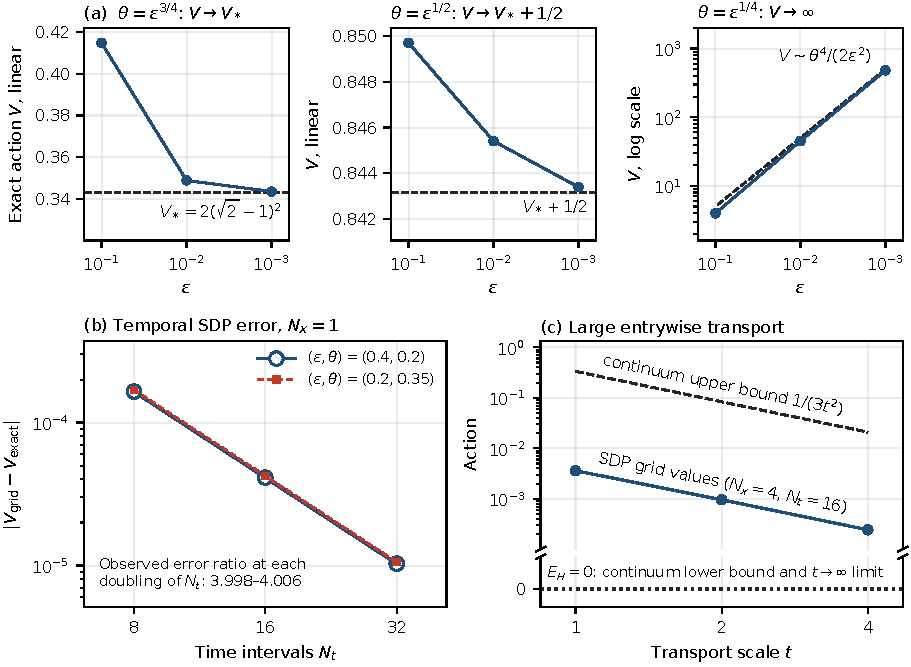
\includegraphics[width=\textwidth]{figures/theory_comparisons.pdf}
\caption{(a) Upper three facets: exact minimum action $V$ of
Proposition~\ref{prop:reactionrotation} for
$\theta=\varepsilon^{3/4},\varepsilon^{1/2},\varepsilon^{1/4}$ at
$\varepsilon=10^{-1},10^{-2},10^{-3}$, on separate vertical axes
(linear, linear, logarithmic). Dashed lines mark the limits
$V_*=2(\sqrt2-1)^2$ and $V_*+1/2$ and the asymptotic reference
$V\sim\theta^4/(2\varepsilon^2)$ of the same proposition.
(b) Absolute differences between SDP values with $N_x=1$ and exact values,
on common axes, for $(\varepsilon,\theta)=(0.4,0.2)$ (circles, solid line)
and $(0.2,0.35)$ (squares, dashed line).
(c) SDP values on the fixed grid $N_x=4$, $N_t=16$ (circles) and the
continuum upper bound $1/(3t^2)$ of Theorem~\ref{thm:hub} (dashed). The
separate linear strip below the axis break marks $E_H=0$ (dotted), the
continuum lower bound and the $t\to\infty$ limit.}
\label{fig:numerical}
\end{figure}
\FloatBarrier

\section{Formal verification and reproducibility}\label{sec:verification}
The GitHub repository at\\
\url{https://github.com/NewAsiaSuperbear/singular-weights-matrix-transport}\\
contains Lean formalizations of
Theorems~\ref{thm:finite}, \ref{thm:ray}, \ref{thm:uniform},
\ref{thm:hub} and~\ref{thm:separation},
Propositions~\ref{prop:reactionrotation}--\ref{prop:operator}, and the
supporting path constructions. They use signed Radon measures, the complete
closed-domain $C^1$ test class and the normalization in \eqref{eq:action}.
The repository's source inventory and verification manifests identify
the proof files by their hashes.
The pinned toolchain is Lean~4.34.0-rc2; its mathlib revision and the checker
versions are specified in the repository's manifests.
The recorded kernel certificate contains the Lean trust-level-zero check
and the independent Nanoda check of the exported declarations and their
complete dependency closures, with \texttt{propext}, \texttt{Classical.choice}
and \texttt{Quot.sound} as the permitted axioms.

The repository's statement map connects the manuscript results to exact
declaration types and source hashes. The numerical code, figure inputs,
recorded results, verification materials and reconstruction instructions
are also available in the repository.

\section{Conclusion}\label{sec:conclusion}
In the signed-Radon framework of Li and Zou \cite{LiZou},
Theorem~\ref{thm:finite} gives stability of extended minimum values for
convergent weights under eventual relative Gram comparison with factors
tending to one. At finite
target cost, the minimum is attained, near-minimizers admit optimal weak-star
clusters, and Frobenius variations vanish in the null directions of the
limiting weights. The fixed-basis, reaction-zero and partial-reaction results
are specializations of this comparison mechanism.

For large transport scalings with fixed reaction weight, the limiting
reaction-channel infimum retains the original finite-baseline class.
Theorems~\ref{thm:ray} and~\ref{thm:uniform} treat fixed, possibly singular
rays and uniform divergence in every direction separately. For entrywise
divergence on a convex domain with positive-definite reaction weight, the hub
construction identifies the latter limit with the weighted Bures value of
the total endpoint matrices and gives an explicit recovery bound.

The rotating families and norm-divergent sequence exhibit failures of value
continuity and of magnitude-based convergence assumptions. The unscaled-flux
example separates convergence of actions from compactness of fluxes. The
Kantorovich--Bures obstruction and smooth positive separation show that the
operator can affect both large-weight limits and costs along a common
weak-star convergent family of uniformly positive densities.

\section*{AI declaration}
Generative AI tools contributed to the mathematical development and the organization and revision of this manuscript. The author provided initial ideas, made substantive contributions to refining the results, reviewed the arguments, and takes full responsibility for the final content.
\bibliographystyle{plain}
\bibliography{references}
\end{document}
